\subsection{Anforderungsanalyse}
\label{subsec:anforderungsanalyse}

Auch wenn die Entscheidung getroffen wurde, das Projekt hybrid und in diesem Rahmen die eigentliche Entwicklung agil umzusetzen ist es dennoch ratsam, eine gewisse Vorarbeit zu treffen um zum einen den Business Case für den Prince2 Rahmen als auch die User Stories für das Product Backlog (siehe ~\ref{subsec:productGoalBacklog}) entwickeln zu können. Im Kontext der Softwareentwicklung wird dieser Prozess als Anforderungsanalyse (Requirements Engineering) bezeichnet. In diesem Prozess werden die Anforderungen erfasst, analysiert, strukturiert und priorisiert. Außerdem werden in dieser Phase erste Spezifikationen festgelegt, die als Rahmen für den weiteren Projektverlauf dienen können.\\

Ebenfalls wichtig ist es, gewisse Abgrenzungskriterien zu erfassen um bereits vor Beginn der Arbeiten sicher festzuhalten, was nicht Ziel des Projekts ist. Auf diese Weise wird zum einen ein sogenannter Scope- oder Featurecreep vermieden, der dafür sorgen würde, dass immer weitere, aber nicht benötigte oder geforderte Funktionalitäten eingebaut werden. Zum anderen wird auf diese Weise sichergestellt, dass plötzliche Anforderungen von Auftraggeberseite aus den ursprünglich definierten Projektrahmen nicht zu stark erweitern.\\

Durch das agile Vorgehen, den iterativ inkrementellen Lieferansatz und den stetig aktualisierten Product Backlog ist hierbei eine detailierte Ausarbeitung nicht so entscheidend, wie bei einem sequentiell durchgeführten Projekt, dennoch ist es ratsam auch hier sorgfältig vorzugehen um späteren Missverständnissen und Verzögerungen vorzubeugen. In einem rein nach Prince2 durchgeführten Projekt ohne eine agile Komponente auf der Lieferebene würden diese Anforderungen in direkt die Baseline einfließen, was zur Folge hätte, dass Abweichungen von dieser Baseline erst nach Genehmigung eines Änderungsantrags durchgeführt werden könnten. Durch das agile Vorgehen wird hier etwas Flexibilität gewonnen, da die Anforderungen in das Product Backlog überführt werden, dass weniger starr aufgebaut ist wie ein Lastenheft, aber dennoch einen konkreten Rahmen benötigt.\\

Das Ziel des ersten Schritts der Digitalisierung der Philetairus Immobilien GmbH wurde nur eine grobe Projektidee umrissen. Gemäß dieser Idee soll ein System für die Abteilung Aussenarbeiten geschaffen werden, welches es Mietern und Eigentümern ermöglicht Meldungen abzusenden, die in das Aufgabengebiet dieser Abteilung fallen (z.B. Schädlingsbefall oder Unkrautwuchs). Neben dem Senden der Meldungen wurde die Verwaltung und Bearbeitung dieser Meldungen als weitere Anforderung genannt. Als Arbeitstitel für das Projekt wurde PhileTipTip gewählt, in Anlehnung an den Warnruf des Siedelwebervogel, der dem Unternehmen Philetairus Immobilien GmbH seinen Namen verliehen hat.\\

Da die geplante Software einen bereits bestehenden Geschäftsprozess unterstützen und optimieren soll, ist es wichtig diesen Prozess so gut wie möglich zu verstehen. Eine Möglichkeit dafür ist das Modellieren eines Geschäftsprozesses, um die Abläufe, Akteure und Zusammenhänge zu erfassen. Diese Modellierung kann dann auch als Grundlage für die Erstellung von UML Diagrammen  für die konkrete Entwicklung verwendet werden.\\

Der Erfassen und Verstehen dieses Prozesses findet in enger Zusammenarbeit mit den Stakeholdern statt, die später die Anwender der zu entwickelnden Software sind. Der Einsatz des im Projekt erstellten Programms soll den bestehenden Prozess so gut es geht optimieren, Redundanzen reduzieren, Reaktionszeiten erhöhen und Fehler vermeiden und auf diese Weise zum einen Kosten senken und zum anderen die Zufriedenheit der Beteiligten am Prozess erhöhen.\\

\newpage

\subsection{Geschäftsprozessmodellierung}

Eine Möglichkeit der Visualisierung ist die Geschäftsprozessmodellierung oder Business Process Modelling, die in natürlicher Sprache die Abläufe des zu beschreibenden Prozesses aufzeigt. Gerade im Bereich der Digitalisierung von Abläufen und Vorgängen ist diese Betrachtung sinn- und wertvoll, da sie zum einen einen konkreten Einblick in die eigentlichen Prozesse schafft und somit eventuelle Optimierungsansätze erkennen lässt und zum anderen für die Entwickler der Digitalisierungslösung einen ersten Überblick gestattet, aus dem Use-Cases und User Stories extrahiert werden können.\\

\begin{figure}[!h]
\centering
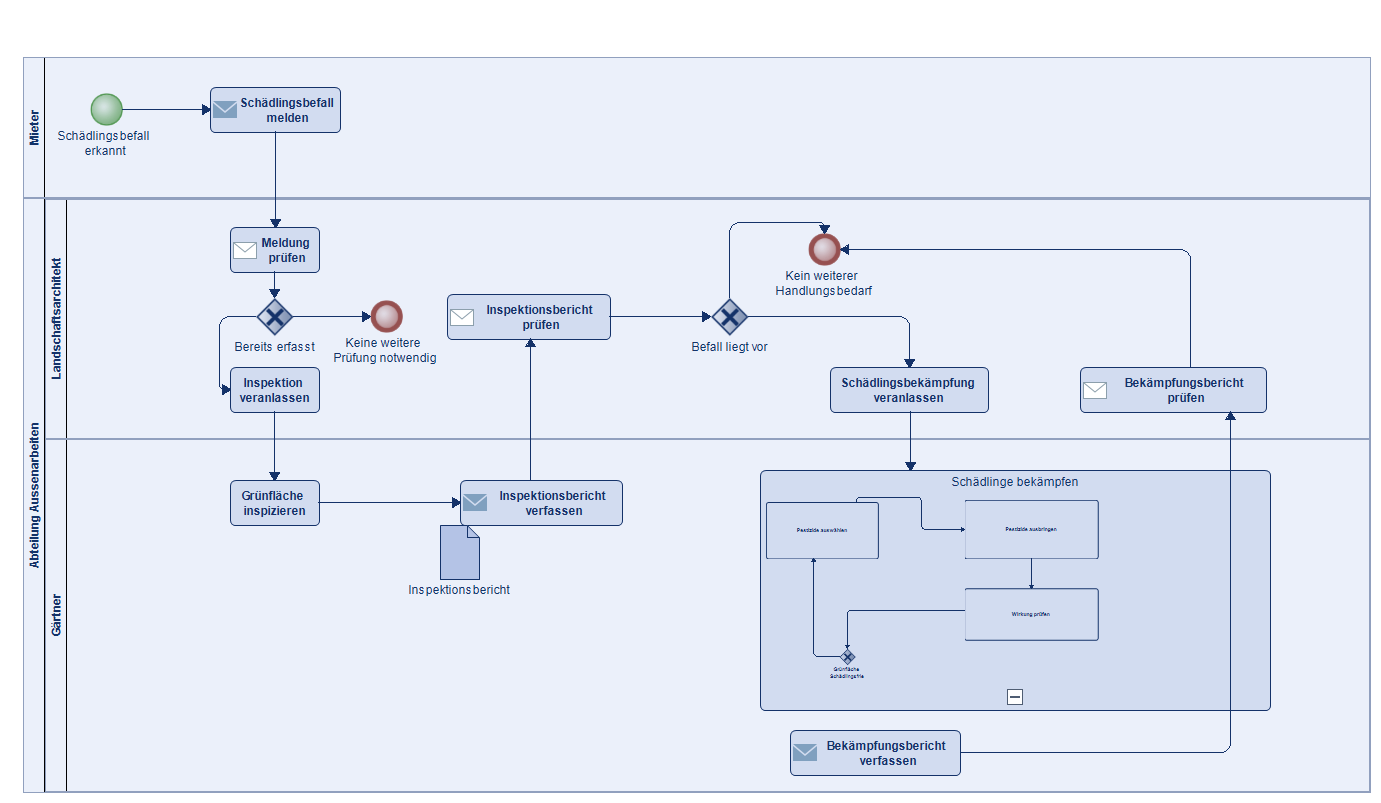
\includegraphics[width=\textwidth]{BPM}
\caption{BPM Diagramm PhileTipTip - eigene Darstellung, erstellt mit Modelio Version 5.4.01}
\end{figure}

Das (vereinfachte) BPM Diagramm stellt den bisherigen Ablauf dar, von der Meldung eines Schädlingsbefalls oder Unkrautbewuchses. Anhand dieser Grafik ist erkennbar, dass es in diesem Prozess viele Optimierungsmöglichkeiten gibt, die sowohl die benötigte Zeit, als auch die an den jeweiligen Schritten beteiligten Akteure reduzieren können. Diese Optimierung entlasten die jeweilige Abteilung, vermeiden Redundanzen und sparen somit Geld und Zeit.\\

Nachdem der Prozess an sich erfasst und verstanden wurde, können die Anforderungen konkretisiert werden. Es ist ersichtlich, dass es drei Hauptakteure gibt, die für die weitere Planung berücksichtigt werden müssen, unter anderem bei der Erstellung von User Stories und Use Cases. Diese User Stories (siehe ~\ref{subsec:userStories}) werden für die weitere Bearbeitung im Product Backlog (siehe ~\ref{subsec:productGoalBacklog}) erfasst und bilden die Basis für den ersten/die ersten Sprints des Scrum Teams.\\

Sowohl die User Stories als auch das Use Case Diagram können und werden sich im Laufe des Projekts (mehrfach) ändern, da es durch das inkrementelle und iterative Vorgehen sehr wahrscheinlich ist, dass einige spezielle Anforderungen und Nutzerwünsche erst ab einem gewissen Entwicklungsschritt ersichtlich werden. Durch die kontinuierliche Kommunikation mit den Endbenutzern ist es möglich, diese während der Entwicklungsphase zu erfassen und umzusetzen.\\

\subsubsection{Funktionale und Nichtfunktionale Anforderungen}

Für gewöhnlich wird in einer Anforderungsanalyse zwischen Funktionalen und Nicht-funktionalen Anforderungen unterschieden. Funktionale Anforderungen beziehen sich auf den Funktionsumfang des Programms, was soll es tun. Nicht-Funktionale Anforderungen können vereinfacht ausgedrückt als Qualitätsanforderungen bezeichnet werden (wie schnell ist der Zugriff, wie sicher die Verschlüsselung, wie stabil die Verbindung etc.).\\

Um die Anforderungen zu erfassen, müssen diese Anforderungen erst gesammelt und erfasst werden (hauptsächlich durch Gespräche mit den unterschiedlichen Stakeholdern). Nach Abschluss dieses Schrittes müssen diese Anforderungen analysiert werden, um sie in eine Hierachie und einen Bezug zueinander zu bringen und zu ermitteln, ob sich einzelne Anforderungen unterstützen (Zielkomplementarität), behindern (Zielkonkurrenz) oder sogar ausschließen (Zielantinomie).\\

%PM_10_Handout_25.06.-09.07.24

Die Funktionalen Anforderungen beantworten die Frage Was das Programm leisten soll.
\begin{itemize}
  \item Erfassung von Meldungen über Schädlingsbefall
  \item Speichern der Meldungen
  \item Anzeige und Sortierung dieser Meldungen
    \item Weiterleitung der Meldungen an die Grünflächenabteilung
    \item Benachrichtigungen an Nutzer über Bearbeitungsstatus
\end{itemize}

Die Nichtfunktionalen Anforderungen beantworten die Frage: Wie soll das Programm diese Anforderungen erfüllen?

\begin{itemize}
  \item Das Business verlangt, dass die Daten On-Premises, also auf Firmeninterner Hardware gehalten werden \cite{onPremise}, nicht aufgrund belastbarer Fakten oder Erfahrungswerte, sondern aufgrund eines starken Misstrauens gegenüber der Cloud Technologie und der Angst vor Kontrollverlust. Von dieser Haltung ist der Projektauftraggeber nicht abzubringen.
  \item  Einfache Bedienbarkeit der App
  \item Leichte Wartbarkeit der App
  \item Leichte Erweiterbarkeit der App
  \item Zuverlässiges Funktionieren der App
  \item Datensicherheit und Datenschutz
  \item Schnelle Reaktionszeiten
  \item Niedriger Datenverbrauch im Mobilbetrieb
\end{itemize}

\newpage

\subsubsection{Verständliche Pläne - Domain Driven Design und Geschäftsprozessmodellierung}

Bei der Erstellung von Individualsoftware ist ein anderes Vorgehen erforderlich als etwa für Standardsoftware, die einen breiten Markt ansprechen und abdecken soll. Durch die Verwendung von Prince2 in Kombination mit Scrum auf der Teamebene ist eine starke Kommunikation zwischen den Auftraggebern/Endanwendern beziehungsweise deren Stellvertretern und den Entwicklern, sowie ein effetkiver Austausch der Entwickler untereinander, ausschlaggebend für den Erfolg.\\

Damit diese Kommunikation effektiv und für alle Stakeholder transparent erfolgen kann, bietet es sich an, hier auf bewährte Diagramme zurückzugreifen, die sämtlichen interessierten Stakeholdern zugänglich gemacht werden können, etwa über einen Information Radiator. Auch wenn nicht beabsichtigt wird, einen vollkommen Modellgetriebenen Ansatz für die Entwicklung der App zu wählen, wird dennoch bereits in der Vorbereitung der Entschluss gefasst, stark auf Modelle und Diagramme zu setzen um die technischen Zusammenhänge für alle Stakeholder schlüssig darzustellen und die logischen Zusammenhänge und Interaktionen der einzelnen Prozesse und Akteure für die Entwickler verständlich zu visualisieren und so eine solide Kommunikationsbasis zu schaffen.\\

Die Möglichkeit noch einen Schritt weiterzugehen als die Modellgetriebene Softwareentwicklung wäre das sogenannte \textit{Domain Driven Design}, auf das in diesem Fall allerdings verzichtet wird, da die Domäne (noch) nicht komplex genug ist um den Aufwand der Modellierung zu rechtfertigen. Allerdings werden (auch durch den agilen Ansatz) viele Kernpunkte dieser Vorgehensweise in die Entwicklung von PhileTipTip einfließen.\\

\newpage
